\chapter{Промышленная и экологическая безопасность}

\section{Анализ опасных и вредных факторов}
При работе на персональном компьютере пользователи подвергаются целому ряду вредных и опасных факторов, которые при несоблюдении установленных норм сказываются на здоровье человека отрицательным образом. Это такие факторы, как: шум, электромагнитные поля, блики и отраженный свет, электрический ток, мерцание изображения, рентгеновское излучение, яркий видимый свет, статическое электричество.

Документом, устанавливающим нормы воздействия вредных факторов при работе с видеодисплейными терминалами (ВДТ) и электронно-вычислительными машинами (ЭВМ), являются СанПиН 2.2.2/2.4.1340-03.

При создании данного программного  продукта помимо ЭВМ использовались ВДТ и принтер. Следовательно, согласно Таблице 1 Приложения 1 СанПин 2.2.2/2.4.1340-03, требуется проконтролировать следующие параметры: уровень ЭМ полей, уровень акустического шума, концентрацию вредных веществ в воздухе, мягкое рентгеновское излучение. Кроме этого следует учесть требования к помещениям, освещению и микроклимату.

\section{Освещение}
Большую часть времени пользователю ЭВМ приходится выполнять зрительную работу. Рабочее место должно удовлетворять нормам освещенности, указанным в СНиП 23-05-95.

На освещенность рабочего места влияют: естественное освещение, искусственное освещение, тон стен и потолка помещения.

Согласно пункту 4.2 СНиП 23-05-95, данная работа относится к работе IV разряда, подразряд в. Параметры и характеристики для данного разряда работ приведены в Таблице~\ref{table:phrz}.

Естественное освещение должно осуществляться через светопроемы, ориентированные преимущественно на север и северо-восток и обеспечивать коэффициент естественной освещенности (КЕО) не ниже 1.5\%.

Искусственное освещение должно осуществляться системой общего равномерного освещения. Освещенность на поверхности рабочего стола должна быть 300-500 лк.

Необходимо ограничивать прямую и отраженную блесткость от источников освещения, что достигается правильным расположением рабочих мест относительно источников освещения. При этом яркость светящихся поверхностей, попадающих в поле зрения, не должна превышать 200 кд/кв.м, яркость бликов на экране ВДТ и ЭВМ не должна превышать 40 кд/кв.м, и яркость потолка при применении системы отраженного освещения не должна превышать 200 кд/кв.м.

В качестве источников света при искусственном освещении должны применяться преимущественно люминесцентные лампы типа ЛБ и компактные люминесцентные лампы (КЛЛ).

При разработке программного обеспечения использовалось помещение с естественной и искусственной системой освещения. На рабочих местах, где проводилась разработка, использовалась естественная боковая система освещения, а также искусственное освещение с применением компактных люминесцентных ламп. При этом оконные проемы располагались слева от рабочих мест, что рекомендуется СанПиН 2.2.2/2.4.1340-03.

\begin{table}
\caption{Параметры и характеристики для разряда зрительных работ IVв.}
\label{table:phrz}
\begin{tabular} {| p{0.15\textwidth} | p{0.15\textwidth} | p{0.13\textwidth} | p{0.21\textwidth} | p{0.1\textwidth} |p{0.15\textwidth} |}
\hline
Наименьший размер объекта различия, мм & Контраст объекта с фоном & Хар-ки фона & \multicolumn{2}{|c|}{Искусственное освещение} & Естественное освещение\\
\hline
 & & & \multicolumn{2}{|c|}{Освещенность, лк} & KEO, \% \\
 \cline{4-6}
 & & & Комбинированное & Общее & Боковое \\
\hline
0.5-1.0 & Малый Средний Большой & Светлый Серый Темный & 400 & 200 & 1.5\\
\hline
\end{tabular}
\end{table}

\section{Статическое электричество}
При работе монитора на экране кинескопа накапливается электростатический разряд, создающий электростатическое поле (ЭСтП). В разных исследованиях при разных условиях измерений значения ЭСтП колебалось от 8 до 74 кВ/кв.м. При этом люди, работающие с монитором, приобретают электростатический потенциал. Разброс электростатических потенциалов пользователей колеблется в диапазоне от -3 до +5 кВ.

Кроме монитора вклад в общее электростатическое поле вносят электризующиеся от трения поверхности клавиатуры и мыши. После работы с клавиатурой электростатическое поле быстро возрастает с 2 до 12 кВ/м. На отдельных рабочих местах в области рук регистрировались напряженности статических электрических полей более 20 кВ/м.

Монитор MacPro удовлетворяет требованиям стандарта ТСО’99 (допустимое значение поверхностного электростатического потенциала должно быть менее 500В). В соответствии с СанПиН 2.2.2/2.4.1340-03 допустимым является значение 500В. Следовательно, проведение дополнительных мероприятий не требуется.

\section{Напряжение в электрической сети}
Электрические установки, к которым относится практически все оборудование ЭВМ, представляют собой большую потенциальную опасность, поскольку в процессе эксплуатации или проведения профилактических работ человек может коснуться частей, находящихся под напряжением. Специфическая опасность электроустановок - токоведущие проводники, корпуса стоек ЭВМ и прочего оборудования, оказавшегося под напряжением в результате повреждения (пробоя) изоляции, не подают каких-либо сигналов, которые могли бы предупредить человека об опасности.

Помещение, в котором проводилась разработка, согласно ПУЭ, относится ко II-й категории - помещение с повышенной опасностью, напряжение в сети составляет 220В, частота переменного тока - 50Гц, поэтому для обеспечения безопасности использовались:
\begin{itemize}
\item Заземление выносного типа, заземлению подлежат корпуса компьютеров и периферийных устройств ($\textup{К}_{\textup{зу}} <= 10\textup{Ом}$, так как N < 100кВА);
\item Двойная изоляция проводников, сопротивление которой, согласно ПУЭ должно составлять 0.5 МОм;
\item Устройства аварийного отключения питания;
\end{itemize}

\section{Электрические и магнитные поля}
Большая часть составных частей ПЭВМ (системный блок, монитор, клавиатура, дисковые накопители, принтер, сканер) являются источником электромагнитных полей. Примерные частоты электромагнитных полей, создаваемых различными устройствами приведены в Таблице~\ref{table:ch_evm}.

\begin{table}
\caption{Частоты ЭМП, создаваемые различными устройствами ЭВМ}
\label{table:ch_evm}
\begin{tabular}{| p{0.5\textwidth} | p{0.5\textwidth} |}
\hline
Источник & Диапазон частот (первая гармоника)\\
\hline
Монитор & до 100кГц\\
\hline
Процессор & до 2000 МГц\\
\hline
Источник бесперебойного питания & 100 кГц\\
\hline
Другие устройства & 50 кГц\\
\hline
\end{tabular}
\end{table}

В Таблице~\ref{table:vrur_evm} приводятся временные допустимые уровни ЭМП, создаваемых ЭВМ.

Как уже выше упоминалось, при разработке и использовании программного обеспечения предусматривается использование монитора, удовлетворяющего требованиям ТСО’99, которые строже требований СанПиН 2.2.2/2.4.1340-03. ЭМ излучение от системного блока экранируется заземленным металическим корпусом. Такие периферийные устройства, как принтер, были вынесены в отдельное помещение.

\begin{table}
\caption{Временные допустимые уровни ЭМП, создаваемые ЭВМ}
\label{table:vrur_evm}
\begin{tabular}{| p{0.4\textwidth} | p{0.3\textwidth} | p{0.2\textwidth} |}
\hline
Наименование параметров & \multicolumn{2}{l |}{ВДУ ЭМП}\\
\hline
Напряженность эл. поля & Диапазон 5 Гц - 2 кГц & 25 В/м\\
\cline{2-3}
& Диапазон 2 кГц - 400 кГц & 2.5 В/м\\
\hline
Плотность магнитного поля & Диапазон 5 Гц - 2 кГц & 250 нТл\\
\cline{2-3}
& Диапазон 2 кГц - 400 кГц & 25 нТл\\
\hline
\end{tabular}
\end{table}

\section{Шум и вибрация}
При постоянной работе на ЭВМ уровень вибрации не должен превышать допустимых норм вибрации. СанПиН 2.2.2/2.4.1340-03 устанавливает следующие предельно допустимые значения вибрации для рабочих мест (Таблица~\ref{table:vibrac}).

\begin{table}
\caption{Допустимые значения вибрации}
\label{table:vibrac}
\begin{tabular}{| p{0.5\textwidth} | l | l |}
\hline
\multirow{3}{\hsize}{Среднегеометрические частоты октавных полос, Гц}
& \multicolumn{2}{l |}{Допустимые значения}\\
\cline{2-3}
& \multicolumn{2}{l |}{по виброскорости}\\
\cline{2-3}
& м/c & дБ\\
\hline
2 & 4.5x10 & 79\\
\hline
4 & 2.2x10 & 73\\
\hline
8 & 1.1x10 & 67\\
\hline
16 & 1.1x10 & 67\\
\hline
31.5 & 1.1x10 & 67\\
\hline
63 & 1.1x10 & 67\\
\hline
Корректированные значения и их уровни, дБ & 2.0x10 & 72\\
\hline
\end{tabular}
\end{table}

К внутренним источникам шума относятся вентиляторы, принтеры и другие периферийные устройства ЭВМ. Мощные источники шума такие как сервера должны располагаться в отдельных помещениях с использованием средств звукоизоляции (звукопоглощающих материалов для облицовки стен и потолка помещения) и толстых перегородок (стен).

К внешним источникам шума можно отнести шум с улицы и соседних помещений. Для снижения шума улицы следует использовать более толстые шумопоглощающие стеклопакеты, а проветривание помещения осуществлять посредством системы кондиционирования. Для уменьшения шума соседних комнат следует использовать облицовку стен звукопоглощающими материалами.

\section{Микроклимат}
Согласно пункту 4.2 СанПиН 2.2.2/2.4.1340-03, в производственных помещениях, в которых работа с использованием ЭВМ является основной и связана с нервноэмоциональным напряжением, должны обеспечиваться оптимальные параметры микроклимата для категории работа 1а и 1б в соответствии с действующими санитарно-эпидемиологическими нормативами микроклимата производственных помещений.

Работа программиста проводится в сидячем положении и не требует физического напряжения (расход энергии не более 120ккал/час), поэтому данный вид работ относится к категории 1а.

Кроме того, допустимые уровни положительных и отрицательных аэроионов в воздухе помещений, где расположены ЭВМ, должны соответствовать санитарно-эпидемиологическим нормам (Таблица~\ref{table:microclim}).

\begin{table}[h]
\caption{Параметры микроклимата}
\label{table:microclim}
\begin{tabular}{| p{0.2\textwidth} | p{0.2\textwidth} | p{0.3\textwidth} | p{0.25\textwidth} |}
\hline
Период года & \multicolumn{3}{c |}{Параметры}\\
\hline
& Температура воздуха, \textdegree C & Относительная влажность воздуха, \% & Скорость движения воздуха, м/с\\
\hline
\multirow{2}{*}{Холодный}
& 22-24 & 40-60 & 0.1\\
\cline{2-4}
& 21-23 & 40-60 & 0.1\\
\hline
\multirow{2}{*}{Теплый}
& 23-25 & 40-60 & 0.1\\
\cline{2-4}
& 22-24 & 40-60 & 0.2\\
\hline
\end{tabular}
\end{table}

Для поддержания уровней в пределах допустимых используются различные системы ионизации воздуха. Помещение, в котором проводились работы, оснащено общеобменной приточно-вытяжной системой вентиляции для обеспечения оптимальной температуры в теплый период и Биполярным ионизатором возду-
ха Янтарь-5А, рекомендованные для использования в жилых помещениях. Таким образом, параметры микроклимата и уровни ионизации воздуха в помещении приведены в соответствие с нормой. (Таблица~\ref{table:ioni})

\begin{table}
\caption{Уровни положительных и отрицательных ионов}
\label{table:ioni}
\begin{tabular}{| l | l | l |}
\hline
\multirow{2}{*}{Уровни}
& \multicolumn{2}{l |}{Число ионов в 1 куб.см воздуха}\\
\cline{2-3}
& n+ & n-\\
\hline
Минимально необходимое & 400 & 600\\
\hline
Оптимальное & 1500-3000 & 3000-5000\\
\hline
Предельно-допустимые & 50000 & 50000\\
\hline
\end{tabular}
\end{table}

\section{Расчет уровня шума в серверной комнате}
В качестве источника шума рассматривается сервер. Схема расположения источников шума представлена на Рисунке~\ref{fig:server_schema}.

\begin{figure}
\caption{Расположение источников шума}
\label{fig:server_schema}
\centering
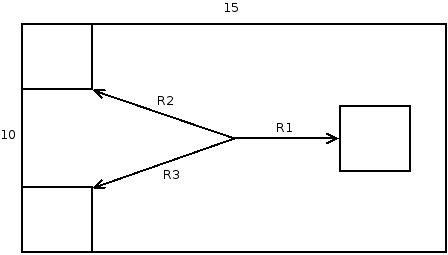
\includegraphics[scale=0.5]{pictures/server_schema}
\end{figure}

Уровни звуковой мощности каждого из источников шума представлены в Таблице~\ref{table:zvuk_power}.

\begin{table}
\caption{Уровни звуковой мощности шума}
\label{table:zvuk_power}
\begin{tabular}{| p{0.1\textwidth} | p{0.15\textwidth} | p{0.12\textwidth} | l | l | l | l | l | l | l | l | l |}
\hline
Источник & Расположение & Расстояние & \multicolumn{9}{c |}{Уровни звуковой мощности, $L_{w}$}\\
\cline{4-12}
& & & 64 & 125 & 250 & 500 & 1000 & 2000 & 4000 & 8000 & S\\
\hline
1 & пол & 5 & 80 & 84 & 83 & 87 & 84 & 82 & 94 & 96 & 157\\
\hline
2 & пол & 5 & 81 & 82 & 83  & 84 & 83 & 81 & 80 & 77 & 39.25\\
\hline
\end{tabular}
\end{table}

Уровни звуковой интенсивности источников шума и расчеты представлены в Таблице~\ref{table:zvuk_results}.

\begin{table}
\caption{Уровни звуковой интенсивности источников шума}
\label{table:zvuk_results}
\begin{tabular}{| p{0.16\textwidth} |  p{0.11\textwidth} | l | l | l | l | l | l | l | l |}
\hline
\multirow{3}{\hsize}{Используемые данные для расчетов}
& Октавные полосы & 63 & 125 & 250 & 500 & 1000 & 2000 & 4000 & 8000\\
\cline{2-10}
& y & 0.8 & 0.75 & 0.7 & 0.8 & 1 & 1.4 & 1.8 & 2.5\\
\cline{2-10}
& B & 30 & 28.125 & 26.25 & 30 & 37.5 & 52.5 & 67.5 & 93.75\\
\hline
\multirow{4}{\hsize}{Номер источника шума}
& 1 & 71.452 & 75.719 & 75.007 & 78.452 & 74.532 & 71.167 & 82.170 & 82.905\\
& & 05 & 94 & 15 & 05 & 17 & 69 & 94 & 16\\
\cline{2-10}
& 2 & 73.008 & 74.245 & 75.500 & 76.008 & 74.210 & 71.071 & 69.280 & 65.334\\
& & 81 & 33 & 75 & 81 & 49 & 85 & 73 & 3\\
\hline
\end{tabular}
\end{table}

Характеристики помещения с источниками шума представлены в Таблице~\ref{table:room_settings}.

\begin{table}[h]
\caption{Характеристики помещения}
\label{table:room_settings}
\begin{tabular}{| l | l |}
\hline
Габариты комнаты & $\textup{м}/\textup{м}^3$\\
\hline
Длина & 10\\
\hline
Ширина & 15\\
\hline
Высота & 5\\
\hline
Объем & 750\\
\hline
\end{tabular}
\end{table}

Предельный спектр уровня шума в помещении с серверами представлен на Рисунке\ref{fig:predel_shum}.

\begin{figure}[h]
\caption{Предельный спектр суммарной звуковой интенсивности в различных октавных полосах}
\label{fig:predel_shum}
\centering
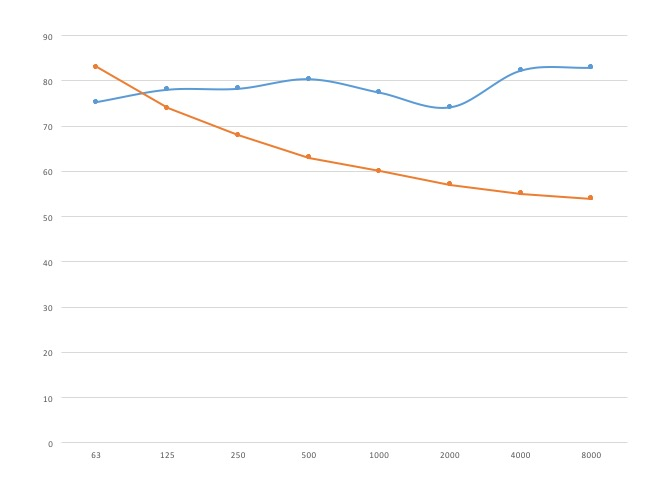
\includegraphics[scale=0.7]{pictures/shum_results}
\end{figure}

Полученные при расчете уровни шума для заданного помещения источников превышают предельно допустимые величины уровней шума. Так как увеличение расстояния от источника до расчетной точки слабо
влияет на уровень шума, а изменение размеров комнаты не снижает уровень шума до допустимых значений, рекомендуется использовать дополнительные методы борьбы с шумом такие как звукоизоляция. Звукоизоляция помещения осуществляется посредством звукоизолирующих материалов, облицовки
стен, кожухов и кабин, заполнением воздушного пространства в двойных
легких перегородках звукопоглощающими материалами, повышением воздухонепроницаемости преграды или применением экранов.

Так как уровни шума превышают допустимые уровни шума, то программисты не должны работать в данном помещении, а во время нахождения рядом с серверами следует использовать индивидуальные
средства защиты (например, беруши).

\section{Утилизация компонентов ЭВМ}
Разрабатываемое программное обеспечение будет использоваться на мощных ЭВМ или серверах. По этой причине встает вопрос о правильной утилизации устаревшего оборудования.

Наибольшую ценность представляют собой различные платы, входящие в состав ЭВМ. В состав утилизированных отходов входят только те платы, которые содержат драгоценные металлы. В современном понимании утилизация отходов представляет собой восстановление ценных материалов путем плавления металлического содержимого, однако стоимость этого процесса такова, что в переработку поступают только платы с очень высоким содержанием драгоценных металлов. Платы, поступающие в переплавку, все без исключения подвергаются обогащению посредством измельчения, а также магнитной и другой дополнительной классификации. Часть отходов, для захоронения которых могла бы понадобиться мусорная свалка, отправляются в Китай для разборки и пиролиза.

Платы с печатными схемами имеют примерный состав материалов, представленный в Таблице~\ref{table:sos_plat}.

\begin{table}
\caption{Состав материалов плат}
\label{table:sos_plat}
\begin{tabular}{| l | l |}
\hline
Стеклополимер & 70\%\\
\hline
Медь & 16\%\\
\hline
Припой & 4\%\\
\hline
Железо, феррит & 3\%\\
\hline
Никель & 2\%\\
\hline
Серебро & 0.05\%\\
\hline
Золото & 0.03\%\\
\hline
Палладий & 0.01\%\\
\hline
Прочие (висмут, сурьма, тантал и т.д.) & <0.01\%\\
\hline
\end{tabular}
\end{table}

Обычно при утилизации используют следующие технологические маршруты:
\begin{itemize}
\item повторное использование компонентов путем их демонтажа;
\item восстановление материалов посредством их механической переработки, пирометаллургии, гидрометаллургии или сочетанием этих технологий;
\end{itemize}

Бракованные платы, отправляемые в плавильную печь, редко подвергаются какой-либо форме обогащения. Производятся только выборочный демонтаж, сортировка и измельчение демонтированных плат. Компании, занимающиеся утилизацией отходов электроники, довольно часто теряют примерно 10\% драгоценных драгоценных металлов, даже применяя процессы флотационного разделения. Потери при переработке плат, содержащих драгоценные металлы в компонентах, составляют примерно 35\%. Известно, что драгоценные металлы в основном присутствуют на выводах компонентов и на контактных площадках плат.

В США и Европе существуют специальные рынки, где продаются демонтированные и восстановленные компоненты плат. Они поступают на рынок с производств, где используют робототехнические системы, обеспечивающие возможность идентификации и демонтажа только тех компонентов, которых не достает на складе. Однако приходится считаться с тем, что быстрое обновление элементной базы и относительно низкая стоимость новых компонентов приведут к серьезному ограничению повторного использования демонтированных компонентов неопределенной давности.

Пиролитическая обработка обычно включает сжигание и плавление размельченного сырья при температуре примерно 1200 \textdegree C. Для этого требуется небольшое количество мазута, так как большая часть энергии обеспечивается за счет сгорания органических компонентов. При этой температуре сгорают органические составляющие отходов, а образующие дымы направляются в камеру дожигания, где они теряют свою токсичность при температуре 1400 \textdegree C. Остающийся от сжигания конгломерат называется "черным металлом". Он, как правило, представляет собой продукт богатый медью. Последующая электролитическая очистка и химическая обработка анодного осадка отделяет медь и другие компоненты от драгоценных металлов.

Новые технологии позволяют не сжигать, а перерабатывать пустые платы в изделия. Например, фирма, FUBA (Германия) перевела на коммерческую основу выделение от 92\% до 95\% металлов из отходов пустых печатных плат за счет использования механических и гидрометаллургических методов разделения. Они включают измельчение, гранулирование, магнитное разделение, классификацию и электростатическое разделение. Совокупность композиций, получаемая от этой обработки, нашла свое применение в изготовлении изделий, имеющих в своем составе большое количество стекловолокна, а также в качестве накопителей в производстве строительных материалов. Особенно успешным оказалось применение стеклополимерных композиций для производства емкостей и поддонов, стойких к химическому воздействию. Металлические составляющие отходов печатных плат (в основном медь) растворяются в таких выщелачивателях, как серная и азотная кислоты, с последующим электростатическим восстановлением меди.

Бракованные печатные платы обычно сортируют по трем категориям, которые отражают количество содержащихся в них драгоценны металлов. Это следующие категории: H - отходы с высоким содержанием драгоценных металлов, M - отходы со средним содержанием и L - отходы с низким содержанием драгметаллов. К H категории относятся дискретные компоненты, интегральные схемы, содержащие золото, устройства оптоэлектроники, платы с содержанием драгоценных металлов, с золоченными и паладированными контактами. Бракованные платы с компонентами по большей части вывозятся в Китай для повторного использования.

Таким образом, процесс утилизации и переработки плат является актуальной темой, а учитывая то, что в состав плат входят драгоценные металлы - является коммерчески выгодным. Это привело к развитию коммерческой инфраструктуры, основанной на сборе печатных плат с последующей их сортировкой по содержанию драгметаллов и восстановлением путем переплавки в плавильной печи. Также появляются новые методы обработки, призванные заменить устаревшие за счет большей эффективности и более дешевой эксплуатации.